\section{Specifications}
\label{sec:specs}
\newcounter{SpecID}

\subsection{Markers}
\refstepcounter{SpecID}
\label{spec:markers}

The arena, and tokens, are labelled with fiducial markers. Each
marker number is associated with a particular feature in the arena,
and also has an associated size.  The marker numbers and sizes are
as follows:

\begin{center}
\begin{tabular}{lcc}
  \toprule
  \textbf{Item} & \textbf{Marker Number} & \textbf{Marker Size (\si{mm})} \\
  \midrule
  Arena boundary & 0 -- 27 & 250 \\
  Central reservation & 28 -- 39 & 250  \\
  % 28 to 31 reserved for robot badges
  Tokens & 100 -- 199 & 80 \\
  \bottomrule
\end{tabular}
\end{center}

\subsection{Arena}
\refstepcounter{SpecID}
\label{spec:arena}

\begin{enumerate}
  \item The arena floor is an \SI{9}{m} $\times$ \SI{9}{m} rectangle. The
        tolerance of these two dimensions is $\pm$ \SI{250}{mm}.
  \item The floor of the arena is carpeted.
  \item The layout of the arena is given in Figure~\ref{fig:arena}. This
        figure is to scale.
  \item The outer walls of the arena are at least \SI{600}{mm} high, and the
        interior surface is white plastic-coated hardboard.
  \item Tokens are placed in a pseudo-random, rotational-symmetrical pattern.
  \item Scoring zones will be bounded by metallic tape around the perimeter
        and internal boundaries.
  \item The raised area is \SI{2.4}{m} $\times$ \SI{2.4}{m} $\pm$ \SI{100}{mm},
        with a height of \SI{180}{mm} $\pm$ \SI{10}{mm}.
  \item Scoring zones for teams will be offset 90\degree anti-clockwise, such
        that a team isn't directly in front of their own scoring zone.
  \item The starting location of the robots is given in Figure~\ref{fig:arena}.
        Teams are allowed to place their robot anywhere such that the entire
        robot is within \SI{1}{m} of the starting point, which will be
        indicated on the floor of the arena. The starting zones are along the
        shorter (\SI{8}{m}) walls of the arena.
\end{enumerate}

\begin{figure}
  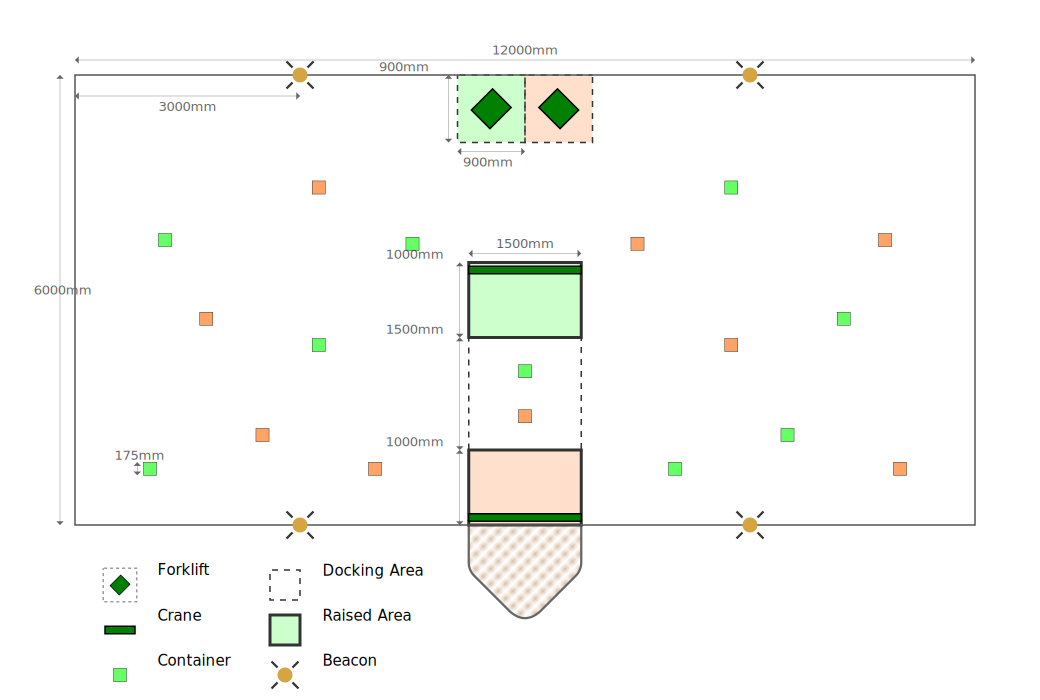
\includegraphics[scale=0.58]{fig-arena.pdf}
  \caption{Layout zones and cans in the arena.}
  \label{fig:arena}
\end{figure}

\subsection{Tin Cans}
\refstepcounter{SpecID}
\label{spec:cans}

\begin{enumerate}
  \item The tin cans are standard 400g steel tin cans, of height \SI{108}{mm}
        ($\pm$ \SI{5}{mm}), and diameter \SI{75}{mm} ($\pm$ \SI{5}{mm}).
  \item The initial layout of tin cans in the arena is given in
        Figure~\ref{fig:arena}.
  \item The tin cans are ferromagnetic.
\end{enumerate}
